\section{Overview of \ac{ML}}

\subsection{Tasks \& learning protocol}

% \begin{frame}[label=Supervised_Learning_1]
%   \note{
%     \begin{itemize}
%     \item Present classic supervised learning
%     \end{itemize}
%   }
%   \frametitle{Supervised learning (1/2)}

%   \begin{textblock}{90}(5,15)
%     % Inspired by figure 3.4 in \cite{barra2021} (p. 82)
%     \begin{tikzpicture}
%       \tikzstyle{line} = [draw, -latex', thick]
%       \def\examples{$\example_1, \example_2, \cdots, \example_{\nTrainingSamples}$}
%       \def\labels{$\knownLabel_1, \knownLabel_2, \cdots, \knownLabel_{\nTrainingSamples}$}
%       \def\predictions{${\footnotesize\apply{\hyp}{\example_1}, \cdots, \apply{\hyp}{\example_{\nTrainingSamples}}}$}

%       % Environment
%       \def\env{Environment}
%       \node[minimum width=2.5cm,ellipse,draw,thick] (\env) at (0, 0) {\env{} $\exampleSet$};

%       % Oracle
%       \def\oracle{Oracle}
%       \node[ellipse,draw,thick,right = 2.5cm of \env] (\oracle) {\oracle{}};

%       % Learner
%       \def\learner{Learner}
%       \node[minimum width=2.5cm,draw,thick,below = 1.5cm of \oracle] (\learner) {\learner{} $\hyp \in \hypSet$};

%       % Output of learner
%       \def\output{Output}
%       \node[right = 0.3cm of \learner] (\output) {\predictions};

%       % \env -> \oracle & \env -> \learner
%       \path[line] (\env) -- node[above=0.2cm] {\examples} (\oracle);
%       \path[line] (\env) -- +(0,-1) |- node[below=0.2cm] {\examples} (\learner);

%       % \oracle -> learner
%       \path[line] (\oracle) -- node[right=0.1cm] {\labels} (\learner);

%       % \learner -> \output
%       \draw[line] (\learner) -- (\output);
%     \end{tikzpicture}
%   \end{textblock}

%   \begin{textblock}{90}(5,55)
%     \begin{itemize}
%     \item The environment generates $\nTrainingSamples$ examples
%       $\drawFrom{\example}{\pdfExample}$ (unknown)
%     \item The oracle labels them according to a function $\targetFunc: \exampleSet
%       \mapsto \labelSet$ (unknown)
%     \item The learner has a set of functions $\exampleSet
%       \mapsto \labelSet$, noted $\hypSet$
%     \item The goal is to find $\opt{\hyp} \in \hypSet$ that approximates
%       $\targetFunc$
%       \begin{itemize}
%       \item Note that it's possible that $\targetFunc \not\in \hypSet$
%       \end{itemize}
%     \end{itemize}
%   \end{textblock}
% \end{frame}


\begin{frame}
  \note{
    \begin{itemize}
    \item Give some details about the tasks
    \item Link to statistics
    \end{itemize}
  }
  \frametitle{Supervised learning}

  \begin{textblock}{90}(5,10)
     \begin{block}{Supervised data}
       \begin{itemize}
       \item Dataset
         $\setpredicate{\couple{\example_{i}}{\knownLabel_{i}}}{i=1..\nTrainingSamples}$
         \begin{itemize}
         \item $\example_i \in \exampleSet$ is the input or example
         \item $\knownLabel_i \in \labelSet$ is the true value or desired output or label
         %\item We assume that there is an unknown relation $÷knownLabel = \apply{\targetFunc}{\example_i}$
         \end{itemize}
       \item The learner must produce a function $\hyp: \exampleSet \mapsto \labelSet$
         such that $\predLabel = \apply{\hyp}{\example}$ is close to the known output
         $\knownLabel$
       \end{itemize}
     \end{block}
  \end{textblock}

  \begin{textblock}{90}(5, 42)
    \begin{block}{Tasks in supervised learning}
      \begin{itemize}
      \item<2-> Classification:
        \begin{itemize}
        \item Binary classification (concept learning): $\card{\labelSet} = 2$
        \item Multi-class classification: $\labelSet = \setext{1,..,\nClasses}$
        \item Multi-label classification (multi-output classification): one input can have
        several classes (potentially a variable number)
        \item Examples: classify an animal into a species, medical diagnosis, tagging text or images
        \end{itemize}
      \item<3-> Regression:
        \begin{itemize}
        \item Linear regression: $\labelSet \subset \setR$
        \item Multi-variate regression: $\labelSet \subset \setR^n$
        \end{itemize}
      %\item<4-> Multi-label classification (multi-output classification): one input can have
      %  several classes (potentially a variable number)
      %  \begin{itemize}
      %  \item Examples: tagging text or images
      %  \end{itemize}
      \item<4-> Ranking
      \end{itemize}
    \end{block}
  \end{textblock}
\end{frame}


% \Begin{frame}
%   \note{
%     \begin{itemize}
%     \item Present unsupervised learning \& link to statistics
%     \end{itemize}
%   }
%   \frametitle{Unsupervised learning}

%   \begin{textblock}{90}(5,15)
%     % Inspired by figure 3.4 in \cite{barra2021} (p. 82)
%     \begin{tikzpicture}
%       \tikzstyle{line} = [draw, -latex', thick]
%       \def\examples{$\example_1, \example_2, \cdots, \example_{\nTrainingSamples}$}
%       \def\labels{$\knownLabel_1, \knownLabel_2, \cdots, \knownLabel_{\nTrainingSamples}$}
%       \def\predictions{${\footnotesize\apply{\hyp}{\example_1}, \cdots, \apply{\hyp}{\example_{\nTrainingSamples}}}$}

%       % Environment
%       \def\env{Environment}
%       \node[minimum width=2.5cm,ellipse,draw,thick] (\env) at (0, 0) {\env{} $\exampleSet$};

%       % Oracle is hidden but we need it for node position
%       \invisible{
%         \def\oracle{Oracle}
%         \node[ellipse,draw,thick,right = 2.5cm of \env] (\oracle) {\oracle{}};
%       }

%       % Learner
%       \def\learner{Learner}
%       \node[minimum width=2.5cm,draw,thick,below = 1.5cm of \oracle] (\learner) {\learner{} $\hyp \in \hypSet$};

%       % Output of learner
%       \def\output{Output}
%       \node[right = 0.3cm of \learner] (\output) {\predictions};

%       % \env -> \learner
%       \path[line] (\env) -- +(0,-1) |- node[below=0.2cm] {\examples} (\learner);

%       % \learner -> \output
%       \draw[line] (\learner) -- (\output);
%     \end{tikzpicture}
%   \end{textblock}

%   \begin{textblock}{90}(5,55)
%     \begin{itemize}
%     \item The environment generates examples
%       $\drawFrom{\example}{\pdfExample}$ (unknown)
%     \item No oracle
%     \item The learner tries to model the environment:
%       \begin{itemize}
%       \item Clustering: find groups in $\exampleSet$
%       \item Density estimation: find $\pdfExample$
%       \end{itemize}
%     \end{itemize}
%   \end{textblock}
% \end{frame}


\begin{frame}
  \note{
    \begin{itemize}
    \item Give some details about the tasks
    \item Link to statistics
    \end{itemize}
  }
  \frametitle{Unsupervised learning}

  \begin{textblock}{90}(5,15)
     \begin{block}{Unsupervised data}
       \begin{itemize}
       \item Dataset $\setpredicate{\example_{i}}{i=1..\nTrainingSamples}$
       \item The learner has to describe $\exampleSet$
       \end{itemize}
     \end{block}
  \end{textblock}

  \begin{textblock}{90}(5, 35)
    \begin{block}{Tasks in unsupervised learning}
      \begin{itemize}
      \item<2-> Clustering: find groups in $\exampleSet$
      \item<3-> Density estimation: estimate $\pdfExample$
      \end{itemize}
    \end{block}
  \end{textblock}
\end{frame}


\begin{frame}{Other levels of supervision}
  \note{
    \begin{itemize}
    \item
    \end{itemize}
  }

  \begin{textblock}{90}(5, 15)
    You can imagine other levels of supervision:
    \begin{itemize}
    \item<2-> Semi-supervised: you have $\ell$ labelled examples and
      $\nTrainingSamples - \ell$ unlabelled examples
      \begin{itemize}
      \item Can you use the unlabelled examples to improve the classification?
      \end{itemize}
    \item<3-> Self-supervised: learn a representation of unlabelled data that is
      useful for later supervised learning
    \item<4-> Reinforcement learning: the learner receive delayed and sparse signal
      from the oracle about his performance
    \item<5-> ... and mix them
      \begin{itemize}
      \item ChatGPT is trained in 3 phases: first in a self-supervised phase
        (predict the next word in a phrase),
        then in a supervised phase (predicting requests) and then with
        reinforcement learning (to avoid some behaviour)
      \end{itemize}
    \end{itemize}
  \end{textblock}

  % \begin{textblock}{90}(5, 85)
  %   \onslide<6->{
  %   The difference between the task, the protocol or the technique
  %   is not always clear
  %   }
  % \end{textblock}
\end{frame}


\begin{frame}{Learning protocol}
  \note{
    \begin{itemize}
    \item Briefly present the notion of learning protocol
    \item Online learning -> gradient descent
    \item Difference with statistics
    \item  ``Learning'' is used in many different ways: the difference between the task, the protocol or the technique
      is not always clear
    \end{itemize}
  }

  \begin{textblock}{90}(5,15)
    \begin{block}{}
      The learning protocol describes the interaction between the learner and the
      environment:
      \begin{itemize}
      \item<2-> Batch learning: the training set $\trainingSet$
        is given in one time
        \begin{itemize}
        \item $\nTrainingSamples$ i.i.d samples
        \item Example: linear regression, SVM
        \end{itemize}
      \item<3-> Online learning: examples are given one by one and the learner
        tries to improve on each
        \begin{itemize}
        \item<4-> Example: the gradient descent we illustrated on the \ac{MLP}
        \end{itemize}
      \item<5-> More complex protocols:
        \begin{itemize}
        \item Active learning: the learner searches for examples (no longer i.i.d)
        \end{itemize}
      \end{itemize}
    \end{block}
  \end{textblock}
\end{frame}

\subsection{Theoretical approaches of supervised learning}

\begin{frame}
  \frametitle{Introduction}

  \begin{textblock}{90}(5,10)
    \begin{itemize}
    \item Several approaches have been developped to understand
      supervised learning
    \item Much less for other cases
    %\item<2-> Reminder: in supervised learning, we want to learn the function
    %  $\targetFunc$ used by the oracle to label the examples \hyperlink{Supervised_Learning_1}{\beamerbutton{Details}}
    \end{itemize}
  \end{textblock}

  \begin{textblock}{90}(5,25)
    % Inspired by figure 3.4 in \cite{barra2021} (p. 82)
    \begin{tikzpicture}
      \tikzstyle{line} = [draw, -latex', thick]
      \def\examples{$\example_1, \example_2, \cdots, \example_{\nTrainingSamples}$}
      \def\labels{$\knownLabel_1, \knownLabel_2, \cdots, \knownLabel_{\nTrainingSamples}$}
      \def\predictions{${\footnotesize\apply{\hyp}{\example_1}, \cdots, \apply{\hyp}{\example_{\nTrainingSamples}}}$}

      % Environment
      \def\env{Environment}
      \node[minimum width=2.5cm,ellipse,draw,thick] (\env) at (0, 0) {\env{} $\exampleSet$};

      % Oracle
      \def\oracle{Oracle}
      \node[ellipse,draw,thick,right = 2.5cm of \env] (\oracle) {\oracle{}};

      % Learner
      \def\learner{Learner}
      \node[minimum width=2.5cm,draw,thick,below = 1.5cm of \oracle] (\learner) {\learner{} $\hyp \in \hypSet$};

      % Output of learner
      \def\output{Output}
      \node[right = 0.3cm of \learner] (\output) {\predictions};

      % \env -> \oracle & \env -> \learner
      \path[line] (\env) -- node[above=0.2cm] {\examples} (\oracle);
      \path[line] (\env) -- +(0,-1) |- node[below=0.2cm] {\examples} (\learner);

      % \oracle -> learner
      \path[line] (\oracle) -- node[right=0.1cm] {\labels} (\learner);

      % \learner -> \output
      \draw[line] (\learner) -- (\output);
    \end{tikzpicture}
  \end{textblock}

  \begin{textblock}{90}(5,65)
    \begin{itemize}
    \item The environment generates $\nTrainingSamples$ examples
      $\drawFrom{\example}{\pdfExample}$ (unknown)
    \item The oracle labels them according to a function $\targetFunc: \exampleSet
      \mapsto \labelSet$ (unknown)
    \item The learner has a set of functions $\exampleSet
      \mapsto \labelSet$, noted $\hypSet$
    \item The goal is to find $\hyp \in \hypSet$ that approximates
      $\targetFunc$
      \begin{itemize}
      \item Note that it's possible that $\targetFunc \not\in \hypSet$
      \end{itemize}
    \end{itemize}
  \end{textblock}
\end{frame}


\begin{frame}
  \frametitle{Loss function, true risk and optimal hypothesis}

  \begin{textblock}{90}(5, 15)
    We want to choose the hypothesis that gives the best result ``on
      average''.
    \begin{block}{Loss function}
      Suppose that we have a loss function $\lossFunc: \exampleSet \times \labelSet \mapsto
      \setR^+$ that evaluates how bad one example is predicted by an hypothesis
      $\hyp \in \hypSet$.
    \end{block}
  \end{textblock}

  \begin{textblock}{90}(5, 37)
    \begin{block}{True risk}<2->
      The expectation of the loss function is called the true risk of $\hyp$:
      \begin{equation*}
        \begin{split}
          \apply{\risk}{\hyp} & = \expectation{\apply{\lossFunc}{\apply{\hyp}{\example}, \predLabel}}\\
                              & = \int_{\example \in \exampleSet, \predLabel \in \exampleSet}
                                \apply{\lossFunc}{\apply{\hyp}{\example}, \predLabel} \pdfExampleLabel \intover{\example} \intover{\predLabel}
        \end{split}
      \end{equation*}
    \end{block}
  \end{textblock}

  \begin{textblock}{90}(5, 67)
    \begin{block}{Optimal hypothesis}<3->
      The optimal hypothesis $\opt{\hyp}$ is:
      \[
        \opt{\hyp} = \argmin_{\hyp \in \hypSet} \apply{\risk}{\hyp}
      \]
    \end{block}
  \end{textblock}
\end{frame}


\begin{frame}{Examples of loss functions}

  \begin{textblock}{90}(5, 15)
    \begin{block}{For classification}
      \begin{itemize}
      \item<2-> 0-1 loss:
        $\apply{\lossFunc}{\apply{\hyp}{\example}, \knownLabel} =
        \begin{cases}
          0 & \text{if $\apply{\hyp}{\example}  =  \knownLabel$} \\
          1 & \text{if $\apply{\hyp}{\example} \ne \knownLabel$}
        \end{cases}
        $
      \item<3-> Logistic loss (probabilistic binary classification): $\apply{\lossFunc}{\apply{\hyp}{\example},
          \knownLabel} =
        -\apply{\log}{\frac{\apply{\hyp}{\example}}{1-\apply{\hyp}{\example}}}$
      \item<3-> Cross-entropy loss (multi-class or multi-label)
      \item<4-> Non-symmetric loss function
      \end{itemize}
    \end{block}
  \end{textblock}

  \begin{textblock}{90}(5, 60)
    \begin{block}{For regression}<5->
      \begin{itemize}
      \item<5-> Squared loss: $\apply{\lossFunc}{\apply{\hyp}{\example}, \knownLabel}
        = \left( \apply{\hyp}{\example} - \knownLabel \right)^2$
      \end{itemize}
    \end{block}
  \end{textblock}
\end{frame}


% Note sure about this
\begin{frame}{Generative \vs{} discriminative}

  \begin{textblock}{90}(5, 15)
    \begin{block}{Three broad approaches}
      We can't find $\opt{\hyp}$ since we don't know $\pdfExampleLabel$.
      We can think of 3 approaches:
      \begin{itemize}
      \item<2-> Generative approach: try to model $\pdfExampleLabel$
        \begin{itemize}
        \item Usually involves Bayesian approaches
        \item You can generate new samples $\couple{\example}{\knownLabel}$
          (hence the name)
        \end{itemize}
      \item<3-> Discriminative approach:
        \begin{itemize}
        \item The oracle can be seen as a PDF: $\condpdfLabelExample$
        \item Try to model this
        \end{itemize}
      \item<4-> Directly look for functions $\exampleSet \mapsto \labelSet$ that
        approximate $\targetFunc$:
        \begin{itemize}
        \item For instance for classification, we can look for planes that
          separate the classes
        \item This is the most common point of view
        \end{itemize}
      \end{itemize}
  \end{block}
  \end{textblock}
\end{frame}


\begin{frame}{\acl{Empirical risk minimization}}
  \begin{textblock}{90}(5, 15)
    We don't know $\apply{\risk}{\hyp}$ so we can't find $\opt{\hyp}$ so we need
    another principle.

    \begin{block}{\acf{ERM}}
      In the discriminative approach, the simplest option is to choose:
      \[
        \estim{\hyp} = \argmin_{\hyp \in \hypSet} \underbrace{\frac{1}{\nTrainingSamples} \sum_{\example_i \in \trainingSet} \apply{\lossFunc}{
            \apply{\hyp}{\example_i}, \knownLabel_i
          }
        }_{\apply{\empRisk}{\hyp, \trainingSet}}
      \]
    \end{block}
\end{textblock}

  \begin{textblock}{90}(5, 45)
    \begin{block}{Questions}
      \begin{itemize}
      \item How to find $\estim{\hyp}$ ?
      \item Is it consistent?
      \end{itemize}
    \end{block}
  \end{textblock}
\end{frame}


% Present the notion of learning algorithm and some broad families of algorithm
\begin{frame}{How to find $\estim{\hyp}$?}
  \note{
    \begin{itemize}
    \item $\hypSet$ is crucial
    \end{itemize}
  }

  % barra2021, p. 17
  \begin{textblock}{90}(5, 15)
    \begin{block}{Learning algorithm}
      A learning algorithm is the procedure used to find $\estim{\hyp}$.
    \end{block}
  \end{textblock}

  % barra2021, p. 21
  \begin{textblock}{90}(5, 35)
    \begin{block}{Family of algorithms}<2->
      Depending on the structure of $\hypSet$, we may think of several broad families:
      \begin{itemize}
      \item<3-> If there is a notion of gradient on $\hypSet$, we can use
        gradient-descent techniques:
        \begin{itemize}
        \item \acl{NN}
        \end{itemize}
      \item<4-> If there is no structure on $\hypSet$, our only option is to explore
        it
        \begin{itemize}
        \item Genetic algorithm
        \end{itemize}
      \item<5-> If there is a (partial) order on $\hypSet$, we can use guided exploration:
        \begin{itemize}
        \item Learning logical formulas
        \end{itemize}
      \item<6-> As a special case, we may not use $\hypSet$ at all but just a
        similarity measure in $\exampleSet$:
        \begin{itemize}
        \item $k$-nearest neighbors
        \end{itemize}
      \end{itemize}
      \end{block}
  \end{textblock}
\end{frame}


\begin{frame}{Consistency of \acs{ERM}}
  \note{
    \begin{itemize}
    \item Talk briefly about the theoretical bounds on ERM
    \end{itemize}
  }

  \begin{textblock}{90}(5, 15)
    The main results of Statistical Learning Theory are:
    \begin{itemize}
    \item<1-> We can characterize $\hypSet$ by a number $d{VC}_{\hypSet}$
      (Vapnik-Chervonenkis dimensions):
      \begin{itemize}
      \item This dimension measures the capacity of functions in $\hypSet$ to
        separate points in $\exampleSet$
      \end{itemize}
    \item<2-> \ac{ERM} is consistent i.f.f $d^{VC}_{\hypSet} < \infty$:
      \[
        \lim\limits_{\nTrainingSamples \to \infty} \apply{\risk}{\estim{\hyp}} = \apply{\risk}{\opt{\hyp}}
      \]
      \[
        \lim\limits_{\nTrainingSamples \to \infty} \apply{\empRisk}{\estim{\hyp}} = \apply{\risk}{\opt{\hyp}}
      \]
    \end{itemize}
  \end{textblock}

  \begin{textblock}{90}(5, 70)
    \begin{itemize}
    %\item<4-> Super-impressive in theory
    \item<3-> Those ideas led to the development of new learning algorithms (SVM)
    \item<4-> In practice, $d^{VC}_{\hypSet}$ is known only in some cases:
      \begin{itemize}
      \item Linear classifiers
      \item \ac{MLP}
      \end{itemize}
    \end{itemize}
  \end{textblock}
\end{frame}


\begin{frame}{Over-fitting}
  \note{
    \begin{itemize}
    \item Explain overfitting
    \end{itemize}
  }

  \begin{textblock}{35}(5, 15)
    \begin{itemize}
    \item<3-> Polynomial regression fit better on $\trainingSet$ than linear regression
    %\item<3-> A larger $\hypSet$ may
    \item<4-> But perform poorly on unseen data
    \item<4-> This is a general phenomenon known as over-fitting
    \end{itemize}
  \end{textblock}

  \begin{textblock}{50}(45, 10)
    \begin{center}
      \only<1>{
        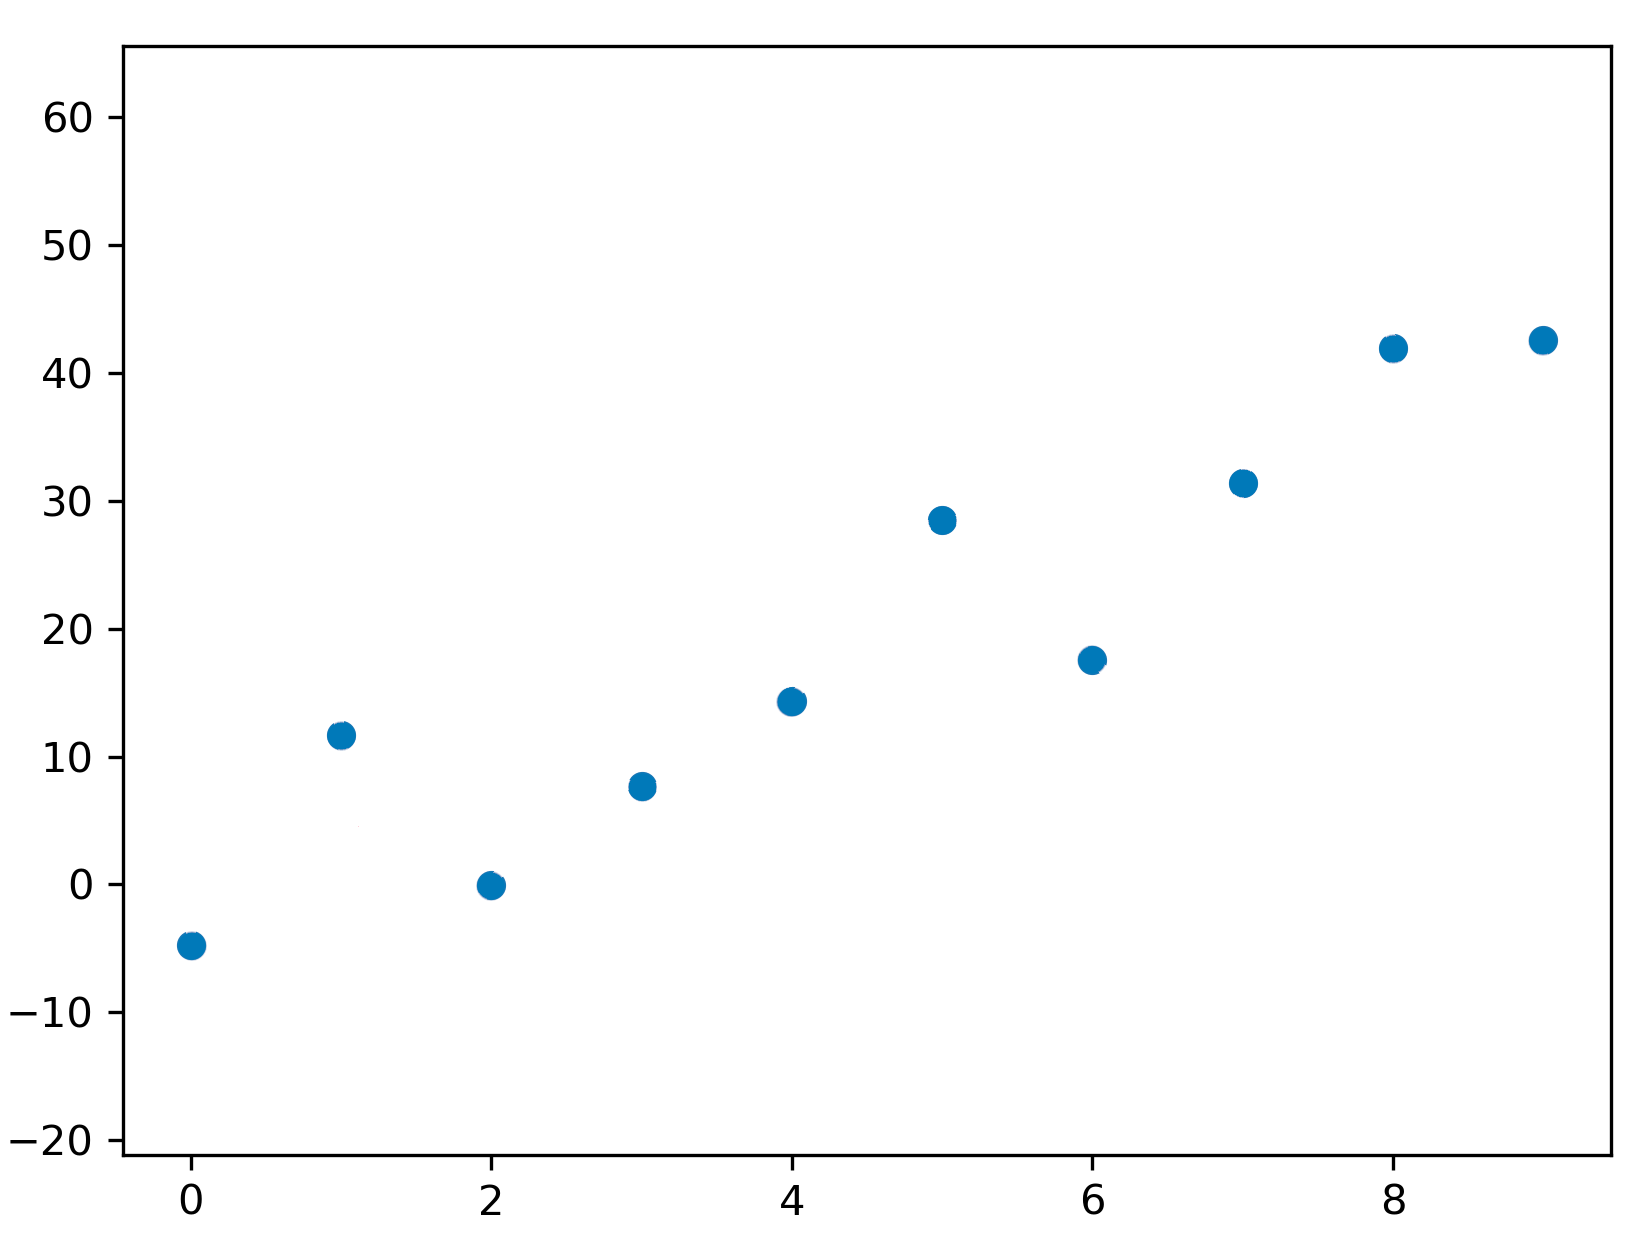
\includegraphics[width=\textwidth]{img/Overfitting_Regression_1.png}
      }
      \only<2>{
        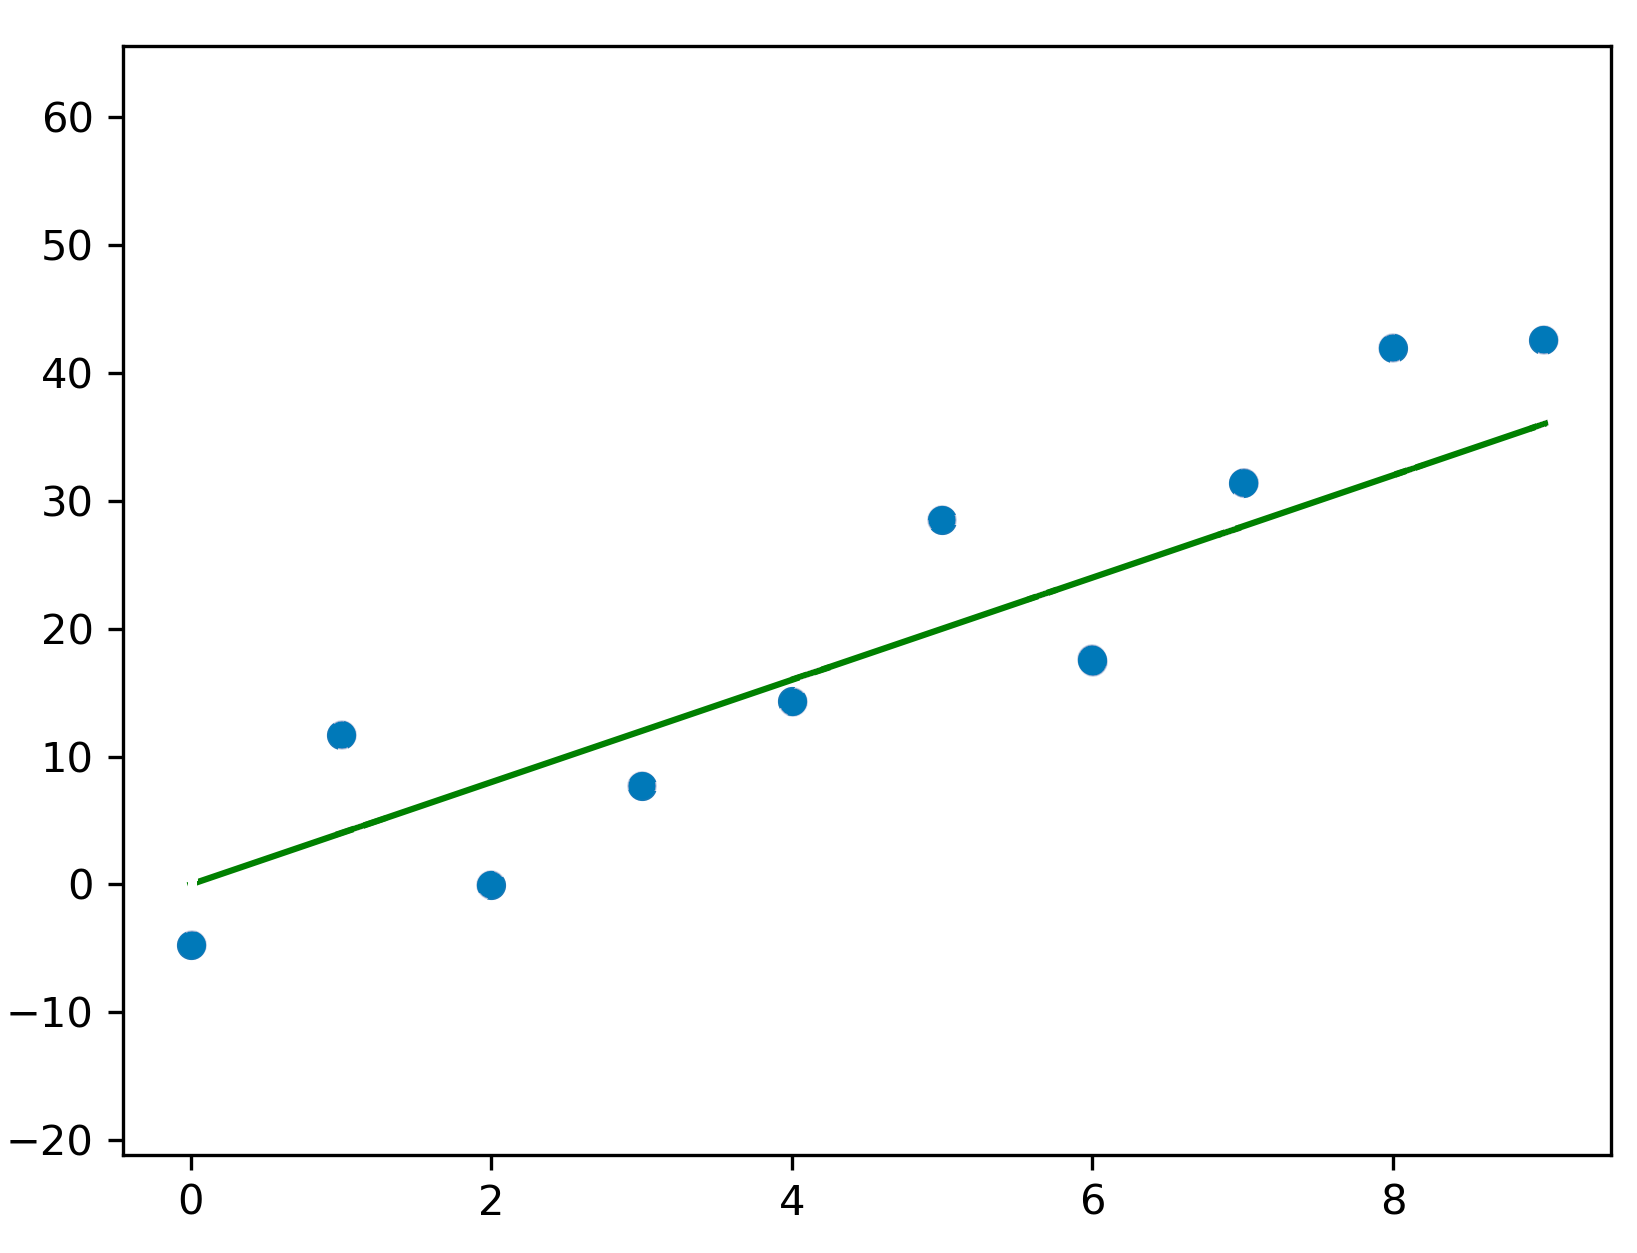
\includegraphics[width=\textwidth]{img/Overfitting_Regression_2.png}
      }
      \only<3->{
        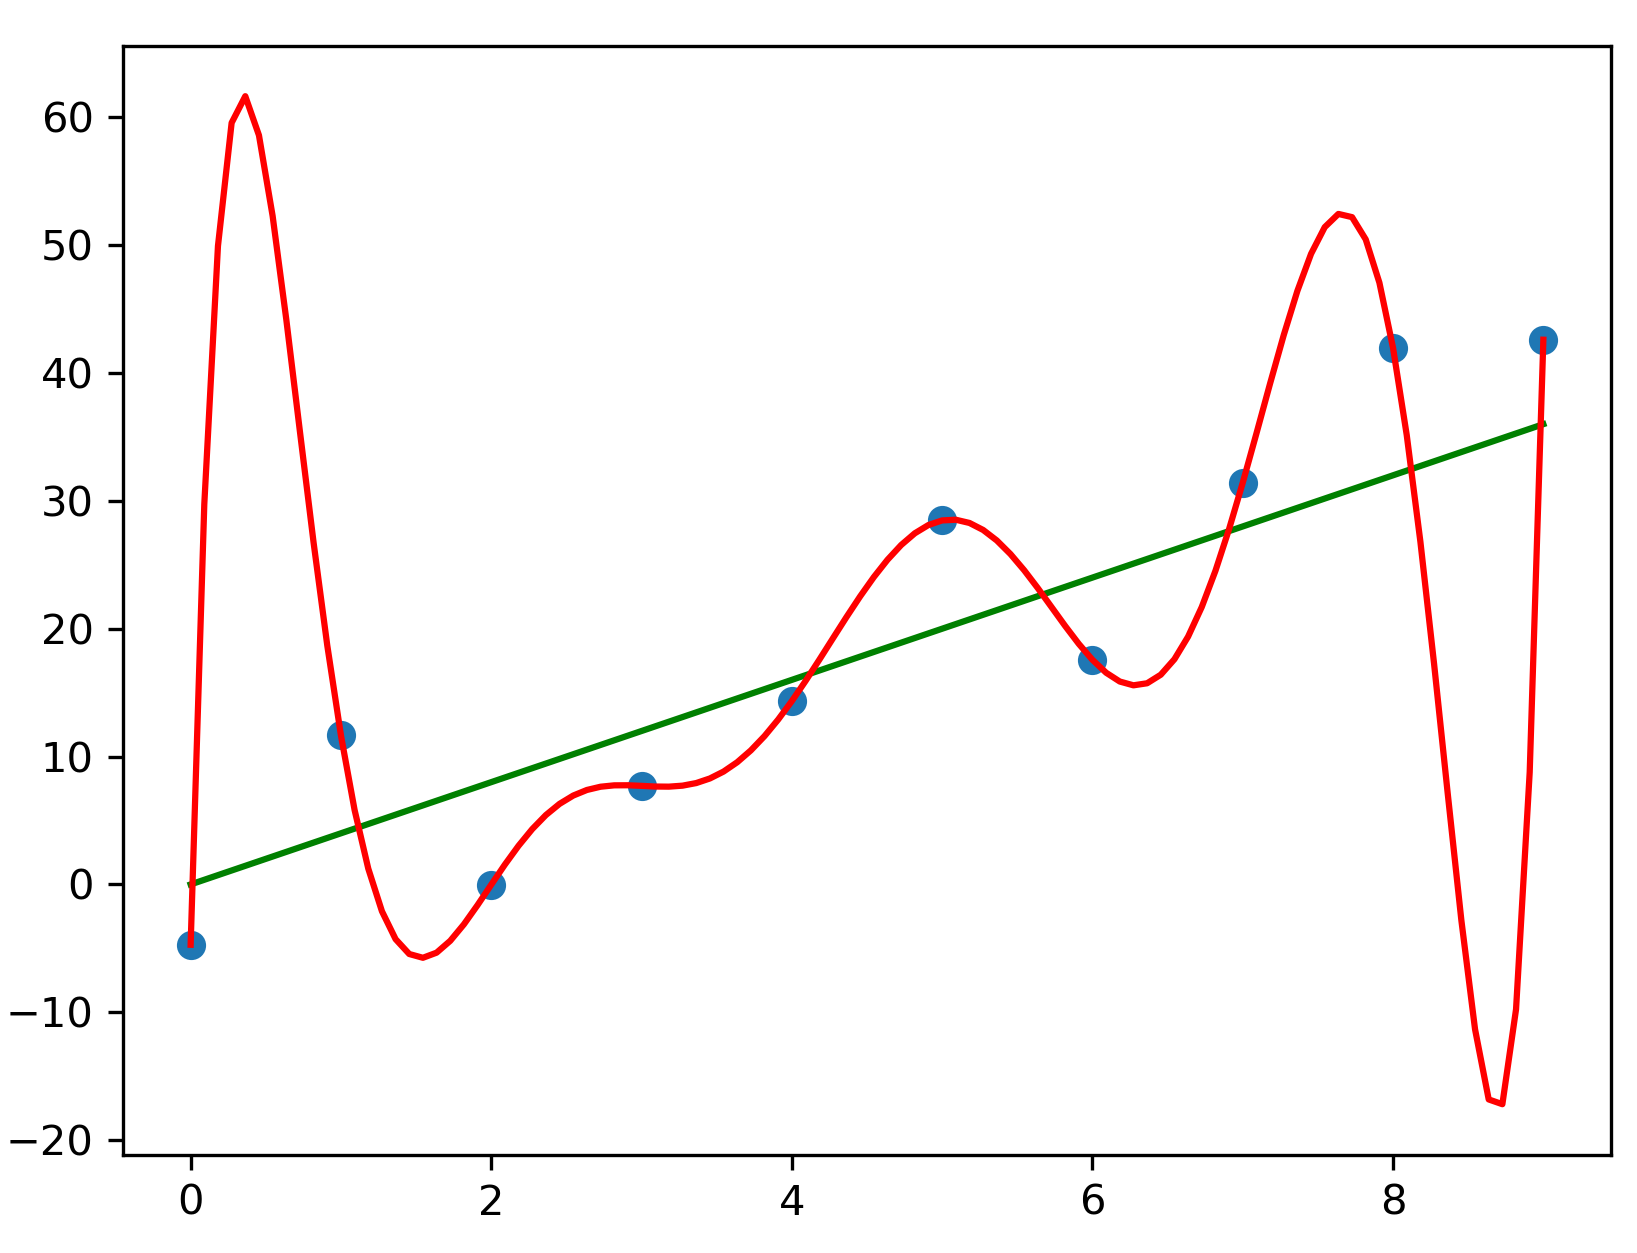
\includegraphics[width=\textwidth]{img/Overfitting_Regression.png}
      }
    \end{center}
  \end{textblock}

  \begin{textblock}{90}(5,65)
    \begin{itemize}
    \item<4-> $\hypSet$ must be chosen according to the problem and
      $\nTrainingSamples$
    \item<5-> You can modify the \ac{ERM} to avoid over-fitting:
      \begin{itemize}
      \item Ideas from Statistical Learning Theory
      \item Penalize ``complex'' models (regularization)
      \item Empirical methods
      \end{itemize}
    \end{itemize}
  \end{textblock}
\end{frame}
